\section{Ein Überblick zu Recommerce und Preisstrategien}
Nicht erst seitdem es Online-Marktplätze gibt, ist die Festlegung von Preisen eine zentrale Herausforderung im Geschäftsbetrieb.
Durch Online-Marktplätze hat allerdings die Intensität des Wettbewerbs erheblich zugenommen, da Konkurrenzangebote leicht einsehbar sind und Preise in hochfrequentem Tempo gesetzt werden können.
Zudem müssen alle Produkte des meist sehr breiten Angebots auf diese Weise mit aktuellen Preisen in Reaktion auf die Marktsituation versehen werden.
Diese Umstände motivieren automatische Preisfindung, da menschliche Branchenkenner mit der Anpassung der Preise schlicht nicht mehr schritthalten können.

Eine weitere Komponente kommt im sogenannten Recommerce hinzu.
Recommerce beschreibt den Rückkauf, die Aufwertung und den Weitervertrieb von gebrauchten Produkten \cite{deges2019grundlagen}.
Gerade mit Blick auf die ressourcenintensive Modebranche verspricht Recommerce eine Steigerung der Nachhaltigkeit durch Einführung einer Zirkularwirtschaft.
Es eröffnet Eigentümern die Möglichkeit, durch den Rückverkauf ihrer nicht weiter benötigten Produkte Geld einzunehmen, und macht Kaufinteressenten gebrauchte und ggf. aufgewertete Produkte zu niedrigeren Preisen verfügbar.
Zur Herausforderung, neue Produkte einzupreisen, kommt also noch hinzu, Preise für gebrauchten Produkte und Rückkaufpreise festzulegen.
Dabei müssen auch Nebenbedingungen wie Lagerkosten beachtet werden, wodurch sich ein durchaus kompliziertes Problem ergibt.
Abbildung \ref{grafic:MarketOverview} zeigt eine grafische Visualisierung des in dieser Arbeit untersuchten Szenarios.

\begin{figure}[htbp]
	\centering
	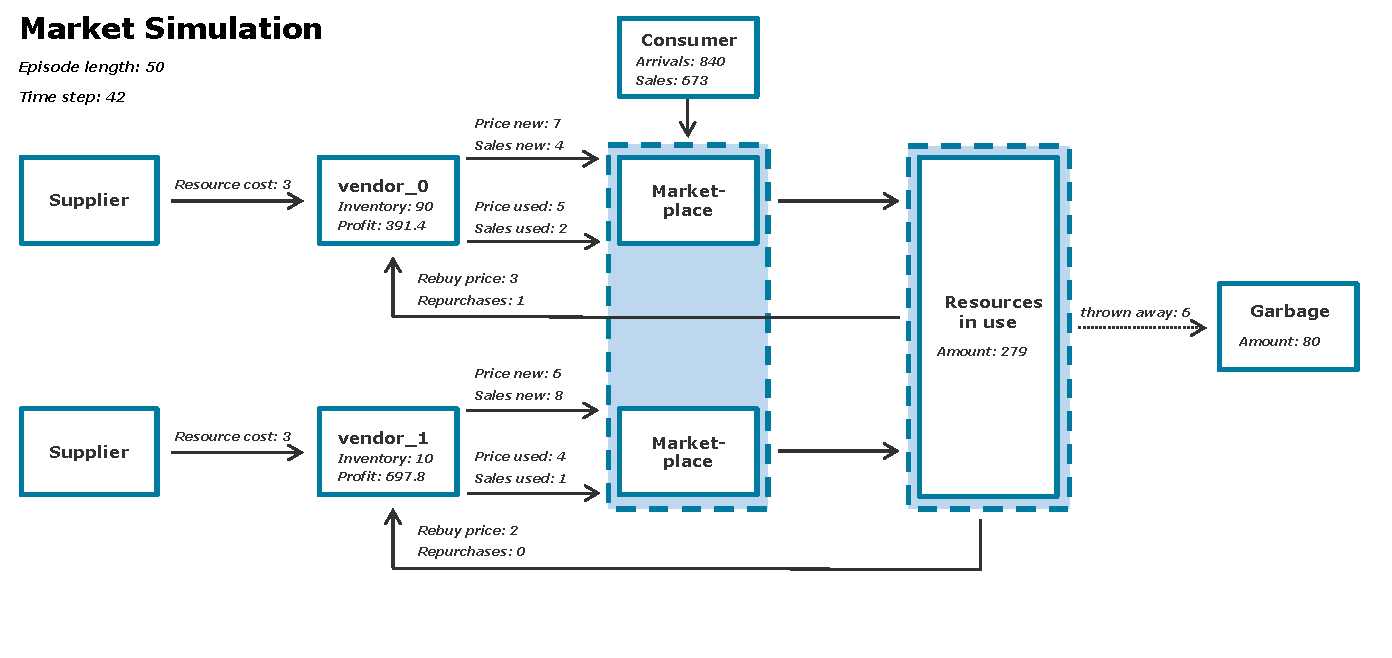
\includegraphics[width=0.85\textwidth]{introduction/MarketOverview_042.pdf}
	\caption{
		Zwei Konkurrenten bieten die gleiche Produktlinie an.
		Beide legen Preise für ihre neuen und gebrauchten Produkte fest.
		Zudem bieten sie Kunden einen Rückkaufpreis für die Rücknahme der gebrauchten Produkte.
		Auch beim Rückkauf gibt es Konkurrenz: Die Eigentümer haben die Wahl, an wen sie zurückverkaufen oder ob sie dennoch wegwerfen.
	}
	\label{grafic:MarketOverview}
\end{figure}

Um das Problem der dynamischen Preisfindung zu lösen, wird das zu untersuchende Szenario zunächst in Abschnitt \ref{section:markov} als Markov-Entscheidungsprozess formalisiert.
Anschließend wird in Abschnitt \ref{section:rulebased} eine regelbasierte Strategie eingeführt.
Der Hauptteil der Arbeit widmet sich allerdings dem Vergleich von Reinforcement-Learning-Verfahren, um die Herausforderung zu meistern.

\section{Der Markt als Markov-Entscheidungsprozess}
\label{section:markov}
Der im vorigen Kapitel intuitiv umrissene Markt wird hier als Markov-Entscheidungsprozess modelliert.
Dazu wird das Marktgeschehen eines geschäftlich relevanten Zeitraumes, z.B. eines Tages oder eines Monats in $n_{ep}$ gleich lange Zeitabschnitte unterteilt.
In der Terminologie des Reinforcement Learnings wird ein einzelner Abschnitt als Schritt, die Gesamtheit als Episode bezeichnet.
Vor jedem Schritt wird dem Agenten der Zustand des Marktes präsentiert.
Das hier eingeführte Modell simuliert einen Recommerce-Markt mit zwei konkurrierenden Anbietern.
Der Markt soll fair und symmetrisch sein, was bedeutet, dass beide Anbieter die gleichen Produkte verkaufen, gleiche Beliebtheit haben, abwechselnd und für die gleiche Länge die Preise setzen und die gleichen Kosten haben.
Damit können die Gewinne der beiden Anbieter direkt verglichen werden und auf die Güte der Preisstrategien geschlossen werden.
Zum Markov-Entscheidungsprozess wird dieser Markt, wenn er aus der Sicht eines der beiden Anbieter betrachtet wird.
Der andere Anbieter wird damit als Teil der Umgebung betrachtet.
Das Verhalten des Konkurrenten kann deterministisch oder stochastisch sein, muss aber für die Markov-Eigenschaft unveränderlich sein.
So werden im Folgenden die Anbieter mit 1 und 2 bezeichnet, wobei 1 der Anbieter ist, aus dessen Sicht das Marktgeschehen abläuft.
Alle Definitionen gelten aber auch analog andersherum.

Jede Preisstrategie muss in Abhängigkeit des Zustandes drei Preise setzen:
\begin{enumerate}
	\item für gebrauchte Produkte der Produktlinie ($p_{1, gebraucht}$),
	\item für diese Produkte in neu ($p_{1, neu}$) sowie
	\item den Rückkaufpreis ($p_{1, re}$), für den von einem Eigentümer gebrauchte Produkte zurückgekauft werden.
\end{enumerate}
Alle drei Preise bewegen sich zwischen 0 und dem maximal möglichen Preis $p_{max}$.
Damit ist der (stetige) Aktionsraum als $\mathcal{A}_\mathbb{R}=[0, p_{max}]^3$ definiert.
Alternativ lässt sich der Aktionsraum auch mit diskreten Preisstufen als $\mathcal{A}_\mathbb{N}=\{0, 1, \ldots, p_{max}\}^3$ definieren.
Die diskrete Formulierung schränkt deutlich stärker ein, ermöglicht aber exakte Lösungen wie im Abschnitt [unten].
Zudem unterscheiden sich die RL-Verfahren für diskrete und stetige Aktionsräume.
Die Preise des Konkurrenten werden als $p_{2, gebraucht}$, $p_{2, neu}$ und $p_{2, re}$ geschrieben.

In jedem Schritt besuchen $k \in 2\mathbb{N}$ Kunden den Marktplatz, betrachten die Angebote und treffen eine von fünf möglichen Entscheidungen.
Entweder kaufen sie kein Produkt, das gebrauchte oder neue beim ersten Anbieter oder das gebrauchte oder neue beim Konkurrenten.
Das Kaufverhalten ist aber keinesfalls deterministisch.
Es wird stark durch die Preise beeinflusst, aber unterschiedliche Kunden haben unterschiedliche Erwartungen, unterschiedliche Konsumgewohnheiten oder unterschiedliche Einstellungen zu Nachhaltigkeit.
Deshalb wird eine Wahrscheinlichkeitsverteilung des Kaufverhaltens über die Kundschaft erstellt, aus der dann für einzelne Kunden geshuffelt wird.
Das geschieht, indem für die einzelnen Optionen Präferenzen aufgestellt werden, aus denen dann per Softmax die Zähldichte der Wahrscheinlichkeitsverteilung berechnet wird.
Die Berechnungsformel für den Präferenzvektor lautet:
\begin{equation}
	\sigma_{kunde}(p_{1, gebraucht}, p_{1, neu}, p_{2, gebraucht}, p_{2, neu}) =
	\begin{pmatrix}
		1\\
		\frac{5.5}{p_{1, gebraucht}} - \exp{(p_{1, gebraucht} - 0.5 p_{max})}\\
		\frac{10}{p_{1, neu}} - \exp{(p_{1, neu} - 0.8 p_{max})}\\
		\frac{5.5}{p_{2, gebraucht}} - \exp{(p_{2, gebraucht} - 0.5 p_{max})}\\
		\frac{10}{p_{2, neu}} - \exp{(p_{2, neu} - 0.8 p_{max})}\\
	\end{pmatrix}
\end{equation}
Die Präferenz für eines der Angebote basiert also hauptsächlich auf dem Preis-Leistungs-Verhältnis.
Gebrauchten Produkten wird dabei 55\% der Wertschätzung im Vergleich zu Neuprodukten entgegengebracht.
Zusätzlich sinkt die Präferenz deutlich, wenn der Preis $0.5 p_{max}$ bei Gebraucht- und $0.8 p_{max}$ bei Neuware überschreitet.
Das modelliert die grundsätzliche Zahlungsbereitschaft der Kunden für diese Produkte und verhindert einen Preiszyklus nach oben.
Wie gefordert, werden die Produkte der beiden Anbieter als gleichwertig betrachtet.
Der Wert 1 als Präferenz für das Nichtkaufen ist festgelegt.
Fallen die Präferenzen der anderen Optionen niedrig aus, so wird durch die Softmax-Funktion eine hohe Wahrscheinlichkeit auf das Nichtkaufen entfallen.
Eine [noch zu erstellende] Darstellung im Anhang veranschaulicht das Kundenverhalten an einigen Beispielen.

Für jeden der beiden Anbieter enthält das Marktmodell einen Zähler für die Anzahl der im Lager befindlichen Gebrauchtprodukte, $n_{lager}$.
Das Lager hat ein Fassungsvermögen von $m_{lager}$ Produkten.
Der initiale Lagerstand wird für beide Anbieter unabhängig und uniform zufällig zwischen $0$ und $m_{lager}$ gewählt.
Wenn mehr Produkte zurücklaufen, werden diese verworfen und der Lagerstand bleibt beim Maximum.
Kauft ein Kunde ein gebrauchtes Produkt, obwohl das Lager leer ist, so muss der Anbieter Entschädigung zahlen.
Die Entschädigung ist auf $2 p_{max}$ pro enttäuschtem Kunden festgelegt.
Das erzeugt einen starken Anreiz für die Anbieter, das Lager nicht leerlaufen zu lassen.
Allerdings verursacht auch die Lagerhaltung Kosten: Am Ende eines jeden Schrittes werden Kosten von $p_{lager}$ pro eingelagertem Element berechnet.
Das wiederum treibt die Anbieter dazu, ihr Lager möglichst klein zu halten und stellt sie vor die Herausforderung, mit dem Rückkaufpreis nicht nur auf ihren Konkurrenten zu reagieren, sondern auch ihr Lager zu regulieren.

Weiterhin verwaltet der Markt einen Zähler für die Anzahl der Produkte, die sich in Zirkulation befinden.
Er wird als $n_{zirk}$ bezeichnet und uniform zufällig zwischen $0$ und $5 m_{lager}$ initialisiert.
Wird ein Neuprodukt gekauft, so wird dieser Zähler um eins erhöht.
Der Kauf von bereits gebrauchten Produkten führt nicht zu einer Erhöhung.
Dieses Modell sieht also nur den einmaligen Weiterverkauf von Produkten vor.

Je mehr Kunden im Besitz eines Produkts sind, desto mehr dieser Eigentümer erwägen, ihr Produkt nicht länger besitzen zu wollen.
Sie stehen in der Zirkularwirtschaft vor einer Entscheidung aus vier Möglichkeiten.
Sie können ihr Produkt weiter behalten, es wegwerfen oder an einen der beiden Anbieter zurückverkaufen.
Die Möglichkeit des Rückkaufs ist nicht auf den Anbieter beschränkt, der ihnen das Produkt ursprünglich verkauft hat, sondern es findet Wettbewerb um den Rückkauf statt.
Insgesamt stellen sich in jedem Schritt $c \cdot n_{zirk}$ Eigentümer dieser Entscheidung, wobei $c$ ein Parameter ist, für den $0 < c \leq 1$ gilt.
Nach dem gleichen Verfahren wie bei der Kaufentscheidung der Kunden wird ihr Verhalten mit einer diskreten Wahrscheinlichkeitsverteilung modelliert, aus der dann für jeden der $c \cdot n_{zirk}$ Eigentümer geshuffelt wird.
Die Berechnung der Präferenzen der Eigentümer geschieht auf Grundlage der Preise der Anbieter mittels dieser Formel:
\begin{equation}
	\sigma_{eigentuemer}(p_{1, gebraucht}, p_{1, neu}, p_{2, gebraucht}, p_{2, neu})=
	\begin{pmatrix}
		1\\
		\min \left(20, \frac{2}{p_{1, gebraucht}},  \frac{2}{p_{2, gebraucht}}\right)\\
		2 \exp{\left(\frac{p_{1, re} - \min{(p_{1, gebraucht}, p_{1, neu})}}{\min{(p_{1, gebraucht}, p_{1, neu})}}\right)}\\
		2 \exp{\left(\frac{p_{2, re} - \min{(p_{2, gebraucht}, p_{2, neu})}}{\min{(p_{2, gebraucht}, p_{2, neu})}}\right)}\\
	\end{pmatrix}
\end{equation}
Sie legt die Präferenz für das Halten eines Produktes auf $1$ fest.
Die Präferenz für das Wegwerfen wird höher, wenn der Gebrauchtpreis niedriger ist.
Die Motivation dazu ist, dass bei einem geringen Kaufpreis der Kunde das Produkt weniger wertschätzt und daher eher geneigt ist, es wegzuwerfen.
Die Präferenzen für das Zurückverkaufen an die jeweiligen Anbieter werden deutlich höher, wenn der prozentuale Unterschied zwischen dem Rückkaufpreis nah am Verkaufspreis ist.
Gedanke dahinter: Die Kunden möchten ihrem Anbieter keine große Rendite zugestehen.
Die Zähldichte der Wahrscheinlichkeitsverteilung ergibt sich dann wieder als Softmax dieser Präferenzen.

Auf einem Online-Marktplatz reagieren die Anbieter gegenseitig auf Preisveränderungen.
Während der erste Anbieter seine Preise stets zu Beginn jedes Schrittes setzt, reagiert sein Wettbewerber in der Mitte eines Schrittes.
Das bedeutet, dass nach stets $k/2$ Kunden die Wahrscheinlichkeitsverteilungen für Kunden- und Eigentümerverhalten neu berechnet wird.
So treffen für jeden Anbieter nach dem Setzen seiner Preise stets $k/2$ Kunden auf das Angebot, das neben den neuen Preisen noch die vorigen des Konkurrenten erhält.
Weitere $k/2$ Kunden treffen dann auf diese Preise und die erneute Reakion des Wettbewerbers.
Einzige Ausnahme ist hier der erste und der letzte Schritt.
Weil der Prozess erst in Gang gesetzt werden muss, muss der Konkurrent den ersten halben Schritt mit Defaultwerten verbringen.
Im Gegenzug wird er bei seinen Preisen im letzten Schritt (die dann noch für einen halben Schritt gelten) keine Preisreaktion mehr bekommen.
Diese Randeffekte fallen jedoch bei den gewählten Episodenlängen nicht ins Gewicht.

Die Belohnung, die der Agent in einem Schritt erhält, ist die Differenz aus Einnahmen und Ausgaben des Agenten in diesem Schritt.
Mit dem Verkauf neuer oder gebrauchter Ware erzielt der Agent Einnahmen.
Ausgaben sind nicht nur der bereits erklärte Rückkaufpreis und die Lagerkosten und -strafen, sondern auch der Einkaufspreis für Neuware.
Pro Neuverkauf zahlt der Agent $p_{einkauf}$.
Damit muss für Gewinn auf dem Bereich der Neuware auf jeden Fall $p_{1, neu} > p_{einkauf}$ gelten.

Nun kann der Zustandsraum des Markov-Entscheidungsprozess $\mathcal{S}$ definiert werden.
Er ist siebendimensional und enthält Folgendes:
\begin{enumerate}
	\item die Nummer des aktuellen Schrittes in der Episode,
	\item die Anzahl der gerade zirkulierenden Elemente,
	\item die Anzahl der Elemente im eigenen Lager,
	\item den Preis des gebrauchten Produkts des Konkurrenten ($p_{2, gebraucht}$),
	\item den Neupreis des Konkurrenten ($p_{2, neu}$),
	\item den Rückkaufpreis des Konkurrenten ($p_{2, re}$) und
	\item den Lagerstand des Konkurrenten.
\end{enumerate}
Diese Werte beeinflussen das Verhalten der Kunden und des Konkurrenten.
Sie müssen gegeben sein, damit die sogenannte Markoveigenschaft erfüllt ist.
Diese besagt, dass die Wahrscheinlichkeiten der Zustandsübergänge und der Belohnungen nur vom aktuellen Zustand und der gewählten Aktion abhängen und damit insbesondere stochastisch unabhängig von den zuvor besuchten Zuständen und Aktionen sind.

Dass die für den Zustandsraum ausgewählten Dimensionen das künftige Verhalten des Systems beeinflussen, ist durch die Definition des Marktverhaltens klar.
So werden Gebraucht- und Neupreis des Konkurrenten noch für die erste Hälfte dieses Schrittes direkt für das Kundenverhalten verwendet.
Der Rückkaufpreis beeinflusst das Verhalten der Eigentümer, deren Anzahl wiederum durch die Anzahl der Elemente in Zirkulation gegeben ist.
Der eigene Lagerstand erklärt durch Lagerkosten- und strafen einen Teil des eigenen Gewinnes, genau wie der Lagerstand des Konkurrenten einen Teil seines Verhaltens erklärt.

Der Schrittzähler als Teil des Zustands verdient noch einmal eine kurze Diskussion.
In zahlreichen Literaturbeispielen wird er nicht benötigt, hier ist er aber wegen der festen Episodenlänge ein Teil des Zustands.
So kann es nämlich einen Unterschied machen, ob man eine ansonsten identische Beobachtung am Anfang oder am Ende einer Episode macht.
Ein Beispiel dafür ist eine Situation mit einem relativ vollen Lager.
Am Anfang kann es sinnvoll sein, einen Teil der Elemente aus dem Lager zu einem niedrigen Preis abzuverkaufen, um langfristig Lagerkosten zu sparen, auch wenn das kurzfristig zu Verlusten führt.
Am Ende ist jedoch kein Raum mehr für langfristige Planung, und es werden hohe Verkaufspreise für kurzfristige Gewinne gesetzt.

Obwohl die Anzahl der zirkulierenden Elemente und der Lagerstand des Konkurrenten für die Markov-Eigenschaft notwendig sind, bereitet die Messung dieser beiden Werte Probleme.
Der Konkurrent lässt sich vermutlich nicht ins Lager schauen und die Anzahl der Elemente in Zirkulation kann allenfalls geschätzt werden.
Deshalb ist es eine zu beleuchtende Frage, ob die untersuchten Verfahren auch mit diesem \textit{partiell beobachtbaren Markov-Entscheidungsprozess} zufriedenstellende Ergebnisse liefern.

Jetzt muss noch einmal beleuchtet werden, dass für den beschriebenen Markt keine weiteren Größen beobachtet werden müssen und somit die Markov-Eigenschaft tatsächlich erfüllt ist.
Das Verhalten des Marktes ist vollständig definiert und kommt mit den genannten Größen aus.
Auch der regelbasierte Wettbewerber in Abschnitt \ref{section:rulebased} verwenden für ihr Verhalten nur die aufgezählten Variablen.
Messgrößen wie die vorher gesetzten Preise, die Anzahl der weggeworfenen Objekte oder die Anzahl der bisherigen Verkäufe könnte man im Zustand vermuten (sie sind ja schließlich auf der grafischen Visualisierung des Marktes), beeinflussen aber nicht das künftige Verhalten.
Eine Gedächtnisfunktion der Kunden (und dann notwendigerweise auch der Agenten) über vergangenes Verhalten ist eine mögliche Erweiterung, die das Modell praxisnäher bringen würde.
So könnten Kunden die vergangene Preispolitik in ihre Entscheidung mit einbeziehen und Anbietern ein höheres oder niedrigeres Renommee zubilligen.
Das erfordert jedoch weitere Techniken, die nicht im Rahmen dieser Arbeit betrachtet werden.

\section{Regelbasierte Strategien -- Benchmark und Wettbewerber}
\label{section:rulebased}
Der heutige Industriestandard für das Dynamic Pricing ist die Festlegung von Regeln durch menschliche Experten.
Sie erstellen Funktionen für die Einpreisung der verkauften Waren, denen prinzipiell die gleichen Argumente wie den RL-Agenten zur Verfügung stehen.
Beim Design dieser Preisstrategien müssen die Herausforderungen des Marktes bereits erkannt sein und für verschiedene Situationen Lösungen vorweggenommen werden.
Für den hier definierten Markt lassen sich einige Überlegungen anstellen:
\begin{itemize}
	\item Die Kunden bevorzugen niedrigere Preise.
	Es erscheint also plausibel, bei Neu- und Rückkaufpreis die Konkurrenz zu unterbieten.
	\item Es sollte allerdings nur bis zu einem bestimmten Preis unterboten werden, weil ansonsten die niedrige Rendite trotz möglicherweise höherer Verkäufe zu wenig Gewinn ermöglicht.
	Insbesondere muss der Verkaufspreis über dem Einkaufpreis liegen.
	\item Das Lager sollte möglichst leer gehalten werden, um dort Kosten zu sparen.
	Allerdings müssen genug Produkte vorrätig sein, um die Kundenwünsche zu erfüllen.
	Mit einem niedrigeren Rückkaufpreis wird das Lager langsamer gefüllt, mit einem niedrigeren Gebrauchtpreis schneller geleert.
	Umgekehrt wird ein höherer Rückkaufpreis und ein höherer Gebrauchtpreis gesetzt, falls das Lager gefüllt werden soll.
	\item Der Rückkaufpreis sollte stets so niedrig sein, wie es auf dem Markt realisiert werden kann.
\end{itemize}
Diese Überlegungen führen zur regelbasierten Strategie $\pi$ mit dem Neupreis:
\begin{equation}
	\pi\left(p_{2, neu}\right)_{neu} = \max{\left(p_{2, neu} - 1, p_{einkauf} + 1\right)}
\end{equation}
Beim Gebraucht- und Rückkaufpreis wird je nach Lagerstand entschieden.
Der Gebrauchtpreis wird in Abhängigkeit des Konkurrenzpreises und des Lagerstandes folgendermaßen gesetzt:
\begin{equation}
	\pi\left(p_{2, gebraucht}, n_{lager}\right)_{gebraucht} =
	\begin{cases}
		p_{2, gebraucht} + 2 & n_{lager} < m_{lager} / 15\\
		p_{2, gebraucht} + 1 & n_{lager} < m_{lager} / 10\\
		p_{2, gebraucht} - 1 & n_{lager} < m_{lager} / 8\\
		p_{2, gebraucht} - 2 & \text{sonst}
	\end{cases}
\end{equation}
Beim Rückkaufpreis werden die gleichen Fallunterscheidungen unternommen und der Preis gesetzt als:
\begin{equation}
	\pi(p_{2, re}, n_{lager})_{re} =
	\begin{cases}
		p_{2, re} + 1 & n_{lager} < m_{lager} / 15\\
		p_{2, re} & n_{lager} < m_{lager} / 10\\
		p_{2, re} - 1 & n_{lager} < m_{lager} / 8\\
		p_{2, re} - 2 & \text{Sonst}
	\end{cases}
\end{equation}
Diese regelbasierte Strategie erreicht in Tests vernünftige Ergebnisse und stellt wegen ihrer kompetitiven Unterbietung durchaus für RL-Agenten eine Herausforderung dar.
Selbstverständlich ist allerdings anzumerken, dass durch weiteres Tuning durchaus bessere Strategien gefunden werden können.
Das erfordert allerdings Aufwand und eine umfangreiche Kenntnis des Marktes.